% -*-latex-*-
\documentclass[a4paper]{llncs}

\usepackage{amstext}
\usepackage{amsmath}
\usepackage{amssymb}
\usepackage{url}
\usepackage{enumerate}
\usepackage{graphicx}
\usepackage{makecell}
\usepackage{listings}
\usepackage{wrapfig}
\usepackage{paralist}
\usepackage{xspace}
\usepackage{color}
\usepackage{times}
\usepackage{proof}
\usepackage{algorithm}
\usepackage[noend]{algpseudocode}
\usepackage{color}
\usepackage{capt-of}

\lstset{
	basicstyle=\ttfamily, 
	commentstyle=\ttfamily,
	showstringspaces=false, 
	escapeinside=``,
}

\usepackage[colorinlistoftodos,bordercolor=white]{todonotes}

%%


%Transition system
\newcommand{\TS}[1]{\ensuremath{\mathcal{T}_{#1}}}
\newcommand{\states}[1]{\ensuremath{\mathcal{C}_{#1}}}
\newcommand{\transitions}[1]{\ensuremath{\mathcal{R}_{#1}}}
\newcommand{\transition}[1]{\ensuremath{\mathit{t}_{#1}}}
\newcommand{\labels}[1]{\ensuremath{\Sigma_{#1}}}
\newcommand{\enable}[1]{\ensuremath{\mathit{en}_{#1}}}
\newcommand{\reachstates}[1]{\ensuremath{\mathit{RS}_{#1}}}

\newcommand{\location}[1]{\ensuremath{\mathit{L}_{#1}}}
\newcommand{\regionstructure}[1]{\ensuremath{\mathcal{S}_{#1}}}
\newcommand{\regions}[1]{\ensuremath{\mathcal{Q}_{#1}}}

%\newcommand{\AP}{\mathit{AP}}

\newcommand{\reaches}{\ensuremath{\leadsto}}

% BIP
\newcommand{\BIP}{\ensuremath{\textsc{BIP}}\xspace}
\newcommand{\bipvar}[1]{\ensuremath{\mathbb{V}_{#1}}}
\newcommand{\varstate}[1]{\ensuremath{\mathbf{V}_{#1}}}
\newcommand{\locs}[1]{\ensuremath{\mathbb{L}_{#1}}}
\newcommand{\locerr}[1]{\ensuremath{\mathbb{L}_{err_{#1}}}}
\newcommand{\ports}[1]{\ensuremath{\mathbb{P}_{#1}}}
\newcommand{\edges}[1]{\ensuremath{\mathbb{E}_{#1}}}
\newcommand{\init}[1]{\ensuremath{\mathbb{I}_{#1}}}
\newcommand{\allports}{\ensuremath{\bigcup_{i = 1}^n{\ports{i}}}}
\newcommand{\bexp}[1]{\ensuremath{\mathcal{F}_{#1}}}
\newcommand{\expr}[1]{\ensuremath{\mathcal{E}_{#1}}}
\newcommand{\compstate}[1]{\ensuremath{\langle l_{#1}, \mathbf{V}_{#1} \rangle}}
\newcommand{\components}{\ensuremath{\mathcal{B}}}
\newcommand{\bipmodel}{\ensuremath{\mathcal{M}_{\BIP}}}
\newcommand{\comp}[1]{\ensuremath{B_{#1}}}
\newcommand{\region}[1]{\ensuremath{\langle l_{#1}, \phi_{#1} \rangle }}
\newcommand{\portid}[1]{{\ensuremath{id({#1})}}}

\newcommand{\variable}[1]{\ensuremath{\mathbb{V}_{#1}}}



%ART
%\newcommand{\region}[1]{\ensuremath{\psi_{#1}}}
\newcommand{\ART}[1]{\ensuremath{\mathbb{T}_{#1}}}
\newcommand{\artnode}[1]{\ensuremath{\mathit{nd}_{#1}}}
\newcommand{\artroot}{\ensuremath{\mathit{Root}}}
\newcommand{\nodes}{\ensuremath{\mathit{Nodes}}}
\newcommand{\artedge}{\ensuremath{\mathit{Edges}}}
\newcommand{\covers}{\ensuremath{\mathit{Covers}}}
\newcommand{\artpath}{\ensuremath{\pi}}
\newcommand{\interpolant}[1]{\ensuremath{\mathbf{I}_{#1}}}
\newcommand{\cex}[1]{\ensuremath{\mathit{cex}_{#1}}}
\newcommand{\leafs}{\ensuremath{\mathit{Leafs}}}


% POR
\newcommand{\enabled}{\ensuremath{\Gamma_{enab}}}
\newcommand{\sset}{\ensuremath{\Gamma_{sim}}}
\newcommand{\pset}{\ensuremath{\Gamma_{per}}}
\newcommand{\aset}{\ensuremath{\Gamma_{amp}}}
\newcommand{\sbset}{\ensuremath{\Gamma_{stub}}}

%
% Useful symbols and abbreviations
%
\newcommand{\Nat}{\mathbb{N}}    % natural numbers
\newcommand{\Real}{\mathbb{R}}   % real numbers
\newcommand{\Int}{\mathbb{Z}}    % integers
\newcommand{\xone}[2]{#1_1,\ldots,#1_{#2}}   % variable range from 1
\newcommand{\xzero}[2]{#1_0,\ldots,#1_{#2}}  % variable range from 0
\newcommand{\CalC}{\mathcal{C}}              % example of caliph C
\newcommand{\setof}[1]{\{#1\}}               % set
\newcommand{\powerset}[1]{2^{#1}}   % power set
\newcommand{\Def}{\stackrel{\mathrm{def}}{=}}   % definition
\newcommand{\mktuple}[1]{\ensuremath{\langle{#1}\rangle}} % tuple definition
\newcommand{\true}{\ensuremath{\mathit{true}}}
\newcommand{\false}{\ensuremath{\mathit{false}}}


% Software model checkers and tools.
\newcommand{\kratos}{\textsc{Kratos}\xspace}
\newcommand{\nusmv}{\textsc{NuSMV}\xspace}
\newcommand{\nuxmv}{\textsc{nuXmv}\xspace}
\newcommand{\mathsat}{\textsc{MathSAT}\xspace}
\newcommand{\dfinder}{\textsc{DFinder}\xspace}
\newcommand{\vcs}{\textsc{VCS}\xspace}


\title{Technical Report \\ Architecture-based Rigorous System Design: \\ An Airplane Engine Control Software Case Study}

%\author{Qiang Wang\inst{1} \and Xudong Tang\inst{2} \and Weikai Miao\inst{2} \and \\ Joseph Sifakis\inst{4,5} \and Geguang Pu\inst{2,3} \and Yongxin Zhao\inst{2}}

%\institute{%
%Chinese Academy of Military Science, China \and
%School of Software Engineering, East China Normal University, China \and
%Shanghai Industrial Control Safety Innovation Technology Co., Ltd, China \and
%School of Computer Science and Engineering, Southern University of Science and Technology, China\and
%Verimag, Universit\'e Grenoble Alpes, France
%}


\begin{document}


\maketitle


\begin{abstract}
In this case study, we apply architecture-based rigorous system design approach to the control software of the airplane engine controller.
Rigorous system design refers to a formal model-based process that leads from requirements to correct implementations.
Architectures are a means for ensuring global coordination properties of system models and thus, achieving design correctness by construction.
%
We implement the architecture diagrams for airplane engine control software in the Behavior-Interaction-Priority (BIP) component-based framework.
We show how to obtain a system model by applying architectures to a set of atomic components.
We also perform deadlock freedom analysis of the resulting system model by using the BIP tool-set and 
additionally validation analysis of our approach by using nuXmv model checker to verify that the safety properties enforced by the architecture are indeed satisfied.
\end{abstract}



\section{Introduction}
\label{introduction}


Design, manufacture and verification of large scale reliable hardware/software
    systems (e.g. cyber-physical systems) remains a grand challenge in system
    design automation~\cite{sifakis2015}.
To address this challenge, the rigorous system design
    methodology~\cite{sifakis13} and the Behavior-Interaction-Priority (BIP)
    framework~\cite{bip11} have been recently proposed.
%
Rigorous system design can be understood as a formal,
 accountable and coherent process for
 deriving correct and trustworthy system implementations
 from high-level specifications.
%
The essential safety properties of the design are guaranteed
 at the earliest possible design phase
 by applying algorithmic verification to the system model,
 and then the system implementation is automatically generated
 by a sequence of property preserving model transformations,
 progressively refining the model with details specific to the target platforms.


BIP is a component-based system design framework,
 coming with a formal language with well-defined semantics
 and a tool chain supporting rigorous system design process.
 The BIP language offers a three-layered modeling mechanism for
  constructing complex system behavior and architectures~\cite{concur16},
  i.e.,  Behavior, Interaction, and Priority.
%
Behavior is characterized by a set of components,
 which are formally defined as automata extended with linear arithmetic.
%
Interaction specifies the multiparty synchronization of components,
 among which data transfer may take place.
%
Priority can be used to schedule the interactions or resolve conflicts
 when several interactions are enabled simultaneously.
%
The key insight underlying this three-layered modeling mechanism is
 the principle of separation of concerns,
 that is, system computation is captured by a set of components,
 and system coordination is modeled by interaction and priority.
%
Moreover, this layered modeling mechanism also benefits
 the formal verification from allowing us to handle the computation and coordination separately.
%
The BIP tool chain supports both algorithmic verification and testing of high-level system designs
 ~\cite{dfinder10,atva15,tgc15}
 and automatic system synthesis of low-level implementations from high-level system designs~\cite{bip-emsoft10}.
 In practice, BIP has been actively used in several applications~\cite{bipapplication12a,bipapplication18}.


The rest of the paper is structured as follows.
%
In Section~\ref{sec:preliminary} and Section~\ref{sec:bip},
 we introduce the preliminaries and the BIP modeling language.
%
In Section~\ref{sec:relatework} and Section~\ref{sec:conclusions},
 we review the most related works and draw some conclusions and outline directions for future work.



\input{rsdBIP}


\section{Case study}
In this section, we will introduce an airplane engine control software case study. Due to its huge scale, we choose one of its subsystem, the PLA signal processing system, as representative. We will give an informal description of it, focusing on its functional structure, properties and conditional constraints. To perform deadlock freedom analysis, we generate a formal system model in BIP. Finally, we provide model verfication and validation for the system above.

\subsection{Informal description}
The Power Level Angle(PLA) signal processing system is part of the Full Authority Digital Engine Control System(FADEC), which provides engine control during flight to achieve stable and transient engine characteristics. The purpose of PLA signal processing system is to convert the obtained throttle stick signal value into the original throttle stick angle value and judge it. If it is judged that there is no fault, then it will return the corresponding value of the PLA signal after processing and set a fault signal to invalid, representing that the system has no PLA signal fault in current period. Otherwise it will return the fault information and set the fault signal to valid. The flow chart of PLA signal processing is roughly as follows:
%Picture TBD

As shown in figure ?, there are three modules in the system. PLA signals will first undergo a BIT Diagnosis module, then be calibrated and converted into physical quantities. After the Extremum and Slope Diagnosis module, it will finally generate the PLA fault signal for output.

The Built-int Test(BIT) refers to the detection and monitoring of the system and its own equipment. In the PLA signal processing system model, the BIT Diagnosis realizes the analog quantity, or periodic fault detection of circuits such as fault location and processing based on the diagnosis results.

The calibration conversion module's function is to collect the signal from signal collector. The arriving signal will be converted to the corresponding engineering value by means of a calibration curve or an index table.

An Extremum/Slope Diagnosis module contains extremum diagnosis and slope diagnosis.The function of extremum diagnosis is to judge whether the current signal is in valid range since the PLA signal processing system cannot handle illegal data. The function of slope diagnosis is to give the constraint of the magnitude of the change between the two adjacent signals.

The three modules introduced above work together for giving a credible output signal. In the next chapter, we will translate this informal model to formal BIP model for further verification and validation. 
\subsection{Formal system model in BIP}
We design our PLA Signal Processing System's BIP model through a combination between series of BIP components with BIP interactions. The block diagram for our system is shown in figure 1.

\begin{figure}[ht!]
	\centering
	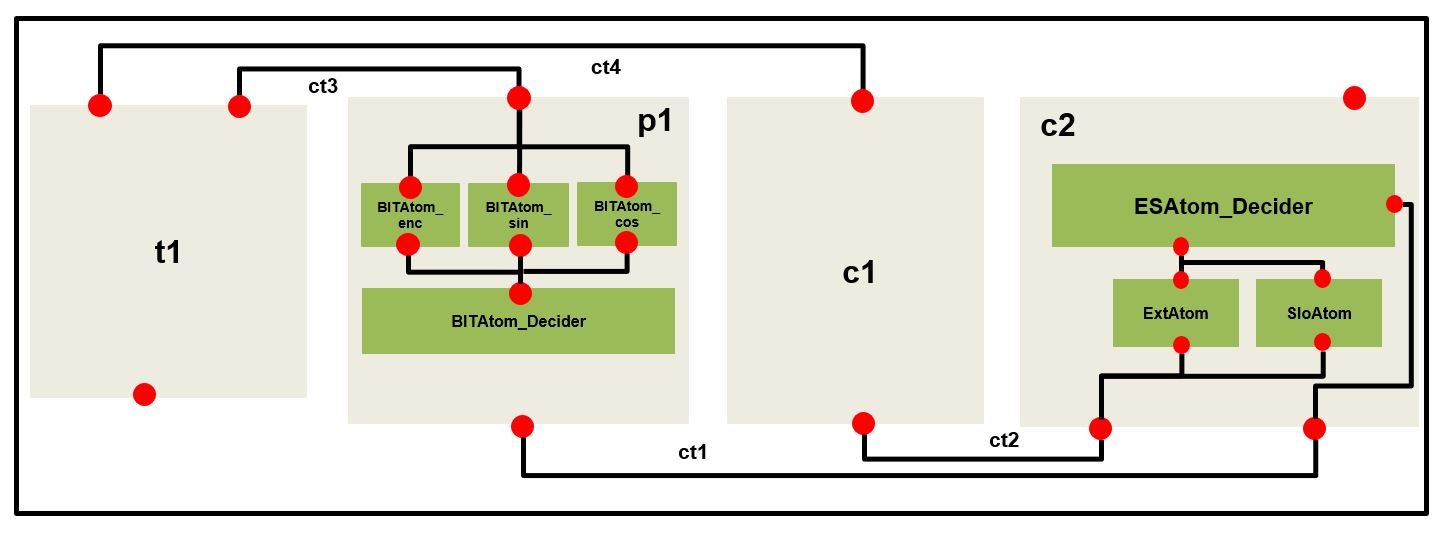
\includegraphics[width=90mm]{figure/figure2.jpg}
	\caption{Architecture of System}
	\label{Sys_Model}
\end{figure}

The atomic components of our system are \emph{TaskAtom t1}, \emph{CalibrationAtom c1} and several atomics in \emph{p1} and \emph{c2}. For each atomic component, we specify its ports, variables and behavior.

\begin{figure}[ht!]
	\centering
	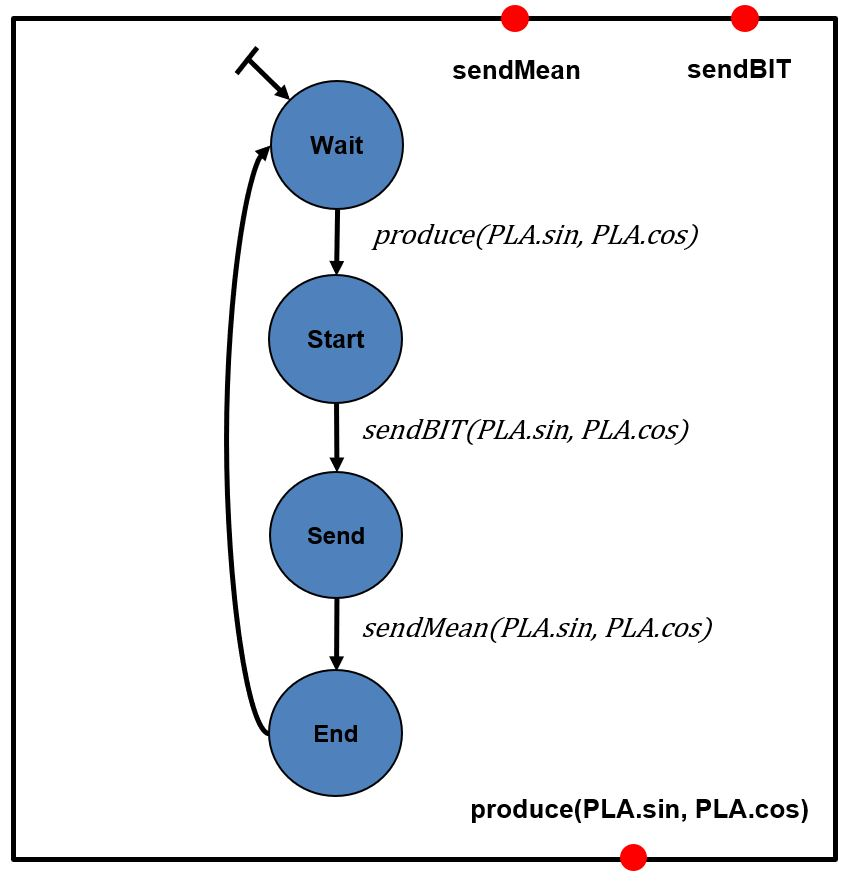
\includegraphics[width=50mm]{figure/figure3.jpg}
	\caption{The Task Component}
	\label{Task_Component}
\end{figure}

\begin{figure}[ht!]
	\centering
	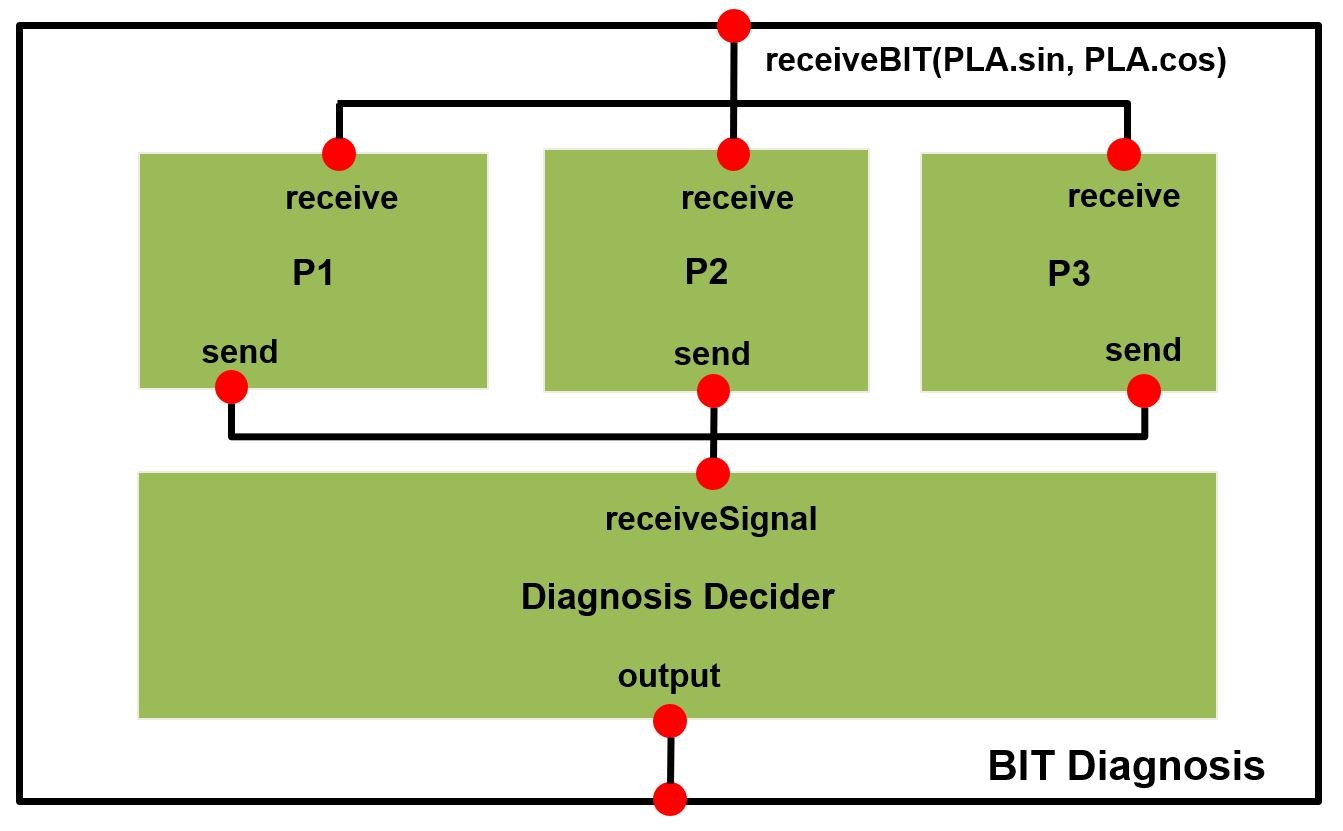
\includegraphics[width=80mm]{figure/figure4.jpg}
	\caption{Architecture of BIT Diagnosis}
	\label{BIT_Model}
\end{figure}

An atomic model of \emph{Task} is shown in figure 2, which can be used as a function of message sender in \emph{System}. In the graphical notation, the atomic is initialized to \emph{Wait}, and the following three transitions are driven by corrensponding events: \emph{produce}, \emph{sendBIT} and \emph{sendMean}, which represents three corrensponding ports in the atomic. For instance, whenever the current state is at \emph{Start}, the port \emph{sendBIT} will be activated and the transition will be executed once the event \emph{sendBIT} is done.

In our design, the BIT Diagnosis is a subsystem of PLA signal processing system. Its architecture is shown in figure 3. In the graphical notation, the three atomic component instances \emph{p1}, \emph{p2} and \emph{p3} receive BIT signal through port \emph{receiveBIT}, a connector distributes the signal to these components and another connector merges their output and sends it to the an instance of \emph{Decider} component. The BIP description of \emph{BIT Diagnosis} is shown below:

\begin{lstlisting}
`\textbf{compound} \emph{BITCompound\_P1}`
  `\textbf{component} \emph{BITAtom\_enc enc}`
  `\textbf{component} \emph{BITAtom\_sin sin}`
  `\textbf{component} \emph{BITAtom\_cos cos}`
  `\textbf{component} \emph{BITAtom\_Decider d}`
  
  `\textbf{connector} \emph{ThreeToOne o(enc.sendBIT,sin.sendBIT,cos.sendBIT,d.receiveSignal)}`
  `\textbf{connector} \emph{Merge m(enc.receiveBIT,sin.receiveBIT,cos.receiveBIT)}`
  
  `\textbf{export port} \emph{m.Merged\_Signal} \textbf{as} \emph{receiveBIT}`
  `\textbf{export port} \emph{d.output} \textbf{as} \emph{sendBIT}`
`\textbf{end}`
\end{lstlisting}

In our system, atomic component is considered as the smallest unit of the architecture, while in the combination of several components, such as our BIT Diagnosis module, we have to ensure that the output of three components can simultaneously reach the connoector, otherwise it will fall into deadlock status. To avoid this problem, the three atomic components are designed homogeneous, we take one of these three components, \emph{BITAtom\_enc p1}, as an example, its ports and behavior is shown below:

\begin{figure}[ht!]
	\centering
	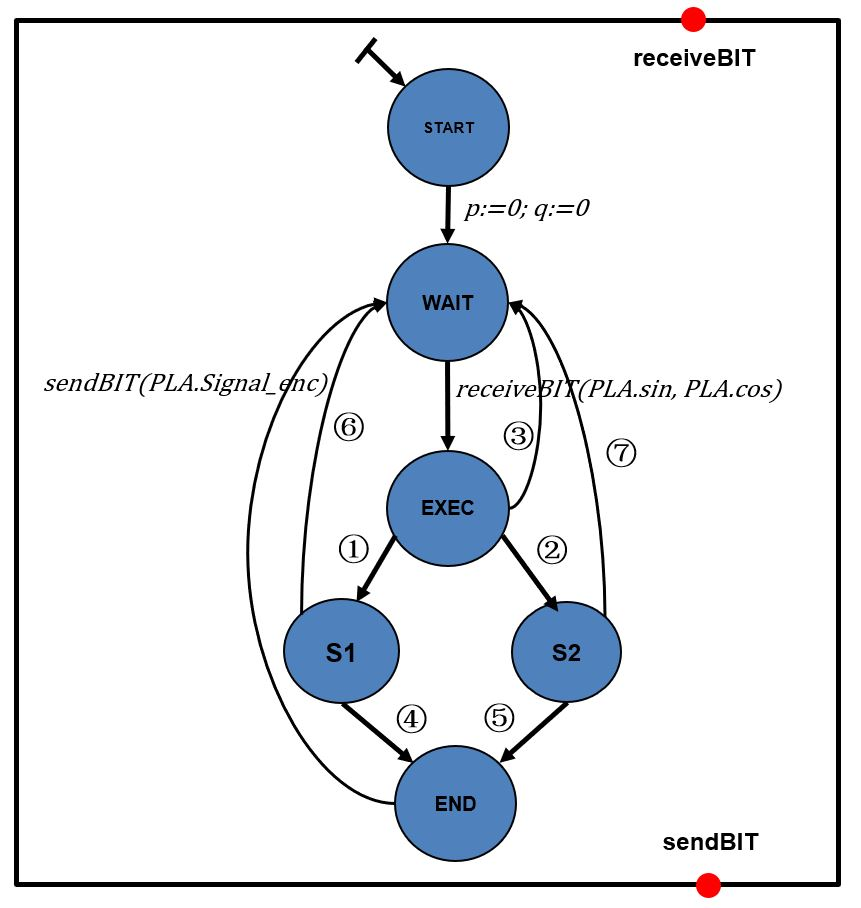
\includegraphics[width=60mm]{figure/figure5.jpg}
	\caption{Architecture of BIT Diagnosis P1}
	\label{BIT_enc_Model}
\end{figure}
\begin{table}[]
	\vspace{20pt}
	\caption{Transitions of P1}
	\centering
	\begin{tabular}{lllll}
		\hline
		\thead[l]{Transition} & \thead[l]{Guard}& \thead[l]{Action}
		\\
		\hline
		1  & PLA.sin $<500 \wedge$ PLA.cos $<500$   & $p :=p+1 ; q :=0$ \\
		2  & PLA.sin $>=500 \wedge$ PLA.cos $>=500$   & $p :=0 ; q :=q+1$ \\
		3  & PLA.sin $ >=500 \oplus$ PLA.cos $>=500$   & $p :=0 ; q :=0$ \\
		4  & $p>=5$   & PLA.Signal\_enc: $=1$ \\
		5  & $q>=5$   & PLA.Signal\_enc: $=0$ \\
		6  & $p<5$   & null \\
		7  & $q<5$   & null \\
		\hline       
	\end{tabular}
	\label{bs}
\end{table}

During execution, we consider a WAIT to WAIT transition set as a cycle. In each cycle, we ensure that an \emph{sendBIT} event will be activated to avoid the system falling into deadlock status. With the combination of connector, \emph{P1} gives a synchronous output together with other two atomic component instances. We define two variables \emph{p} and \emph{q} as counters to control the vary of signal. Their constraint indicates that for every continuous five cycles, the system does a setting and gives a corresponding output through port \emph{sendBIT}.

To give a formal proof of its safety and effectiveness. The verification and validation of the system above will produced in the next chapter.
\subsection{Model verification and validation}





\section{Related work}


In the BIP framework, DFinder~\cite{dfinder10} is a dedicated tool for invariant generation and deadlock-freedom detection.
%
DFinder computes the system invariant in a compositional manner:
it first computes a component invariant over-approximating the reachable states of each component
and then computes an interaction invariant over-approximating the global reachable states.
The system invariant is then the conjunction of all component invariants and the interaction invariant.
%
Though being scalable for large system models,
DFinder does not handle system models with data transfer,
which hampers the practical application of DFinder and of the BIP framework,
since data transfer is necessary and common in the design of real-life systems (e.g. message passing).
%
Besides, it is not clear in DFinder how to refine the abstraction automatically
when the inferred invariant fails to justify the property.

A compositional encoding of BIP into nuXmv
 and an efficient instantiation of Explicit Scheduler Symbolic Thread (ESST) framework for BIP have been presented in~\cite{atva15}.
 The encoding into nuXmv allows one to exploit the state-of-the-art verification techniques to verify BIP models.
%
The ESST based technique encodes the components as preemptive threads with predefined primitive functions and
 utilizes a dedicated stateful BIP scheduler to orchestrate the abstract reachability analysis of the components.
 The scheduler interacts with components via primitive functions, and also respects BIP operational semantics.
 Moreover, partial order reduction techniques are applied in the scheduler to reduce the states of scheduler.

In~\cite{tgc15}, we present a lazy predicate abstraction technique for BIP, and
 we also propose a novel reduction technique called simultaneous set reduction,
 which is further combined with lazy abstraction to reduce the search space of the abstract reachability analysis.


\section{Conclusion and future work}



\bibliographystyle{splncs03}
\bibliography{main}

%\clearpage
%\appendix

\end{document}
